%\section{Implementation and detailed design}
\chapter{Implementation and detailed design}

Present implementation details, program structure etc.

Further, interesting algorithms and data structures should be presented here.

\subsection{Game loop}
Essentially the game is one long loop, which ends whenever the game does.
Each iteration executes the gamelogic per frame, such as moving the player
and monsters around. Gameloops vary from simple while(true) loops to dynamic
separate gameloops handling separate calculations (such as separating rendering
from gameplay).For this we only needed a simple game loop, updating the world in
each iteration. To ensure a consistent gameplay experience, we needed to know how
much time passes betweenframe updates. Without this, the game would run faster
or slower on different processors or inconsistently in different ingame events,
throwing off the players’ sense of timing. For example, the game would be equally
playable with either 30 or 60 frames per second. If the difference isn’t incorporated
in the gamelogic though,the game would run twice as fast with 60 frames per second!
Our implementation of a frames per second counter, is simply calculating how many
frames was calculated the last frame, and then assuming the next frame has the same
amount. This is a pretty simple solution, which could easily be expanded upon if needed.
The obvious criticism of this method, is that the frame calculations between each second
are not accounted for, and that the framerate is essentially a second behind any
framerate changes.

\subsection{Movement}
The movement of our hero will mainly be right and left.
He will have also have the ability to jump. Beside the basics movements,
our hero will also have fight moves. The fight moves contains moves like
sword swinging and archery.

\subsubsection{Input}
The Gameduino 2 comes with a touch screen and accelerometer.
These modules gives us an opportunity to interact with the game
in many ways. We could use the accelerometer or the screen to
move the hero. We don’t have much experience with the screen
and its capabilities. Therefore another option as backup is preferable.

Another option will be using an external controller. The Wii nunchuck is popular and is very suitable for this game.  Using the buttons we game can be controlled as seen in the figure below.


\begin{figure}[h]
  \centering
  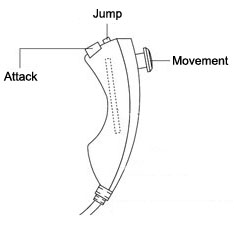
\includegraphics[scale=0.6]{Figures/nunchuk}
  \caption{Button specifications}
\label{fig:Nunchuk}
\end{figure}
